\documentclass[a4paper,11pt]{article}

\usepackage[margin=3cm]{geometry}

\usepackage{graphicx}
\usepackage{subcaption}
\usepackage[colorlinks,allcolors=violet]{hyperref}
\usepackage{url}
\usepackage{lmodern}
\usepackage[dutch]{babel}

% https://tex.stackexchange.com/questions/94032/fancy-tables-in-latex
\usepackage[table]{xcolor}
\usepackage{booktabs}

\usepackage[utf8]{inputenc}

% https://tex.stackexchange.com/questions/664/why-should-i-use-usepackaget1fontenc
\usepackage[T1]{fontenc}
\usepackage{microtype} % good font tricks

\newcommand{\note}[1]{{\colorbox{yellow!40!white}{#1}}}
\newcommand{\exampletext}[1]{{\color{blue!60!black}#1}}

\begin{document}

\noindent
\colorbox[HTML]{52BDEC}{\bfseries\parbox{\textwidth}{\centering\large
  --- Verslag P\&O CW 2019--2020 Taak 3 ---
}}
\\[-1mm]
\colorbox[HTML]{00407A}{\bfseries\color{white}\parbox{\textwidth}{
  Department Computerwetenschappen -- KU Leuven
  \hfill
  \today
}}
\\

\smallskip

\noindent
%\mbox{}\hfill
\begin{tabular}{*4l}
\toprule
\multicolumn{2}{l}{\large\textbf{Team 12}} \\
\midrule
Toon Sauvillers & 60h \\ % fill in the time spend on this task per team member who worked on it
Seppe Van Steenbergen & 54h \\
Bert Van den Bosch & 52h \\
Frédéric Blondeel & 20h \\
\bottomrule
\hline
\end{tabular}\\

\noindent
{\color[HTML]{52BDEC} \rule{\linewidth}{1mm} }

\section{Introductie}\label{sec:introductie}
Het herkennen van schermen, deze identificeren, lokaliseren uit een foto. Dit verslag behandeld deze uitdagingen. Het zoeken van schermen begint bij een foto. Deze foto bevat een scherm met een bepaald uitzicht, er is gekozen voor een groen-blauwe rand waarop gefilterd kan worden. Vervolgens zoekt het algoritme in de gefilterde foto naar aparte schermen en geeft aan hen een id. Met behulp van het kleurenverschil en bepaalde hoeken wordt de oriëntatie bepaald.

Het identificeren van het scherm gebeurd op dit moment nog apart met een kleurenbarcode. Deze barcode bevat 5 verschillende kleuren waardoor er 120 verschillende schermen geïdentificeerd kunnen worden. In de volgende weken worden deze twee, lokaliseren en identificeren, bij elkaar gezet.
\\
Dit verslag behandeld de keuzes die gemaakt zijn alsook een uitleg bij de gebruikte algoritmen en hun tijdscomplexiteit. De mogelijke beperkingen worden met deze kennis geduid.
% The communication protocol should accommodate for:
% \begin{itemize}
%     \item The transmission of images from the smartphone camera to the master.
%     \item Manipulation of the background color of the client screens.
% \end{itemize}
% We are developing a game that requires two players who engage in a confrontation to take a mug shot picture of each other.
% Our game rules will positively encourage both players to provide clean pictures.
% This turned out to be essential since the DeepFace neural network \cite{website:facerecognizer} that we use was not accurate enough in the other scenario's we tested.
% Our analysis of the recognition rate is given in \S\ref{sec:technical-analysis}. Our systematic tests showed we have less than $1\%$~probability of not identifying the correct user out of our test database with $1000$ representative mugshot pictures.

% One unforeseen side effect of the usage of the DeepFace~\cite{amos2016openface} algorithm is the high power consumption.
% We had to balance the performance of the face recognition with battery life time. This was most significant for our indoor game play. In a test run we estimated that the average mobile phone from the supported types will be capable of playing for about $4$~hours and in that time frame scanning and identifying $60$~pictures per hour, see \S\ref{sec:technical-analysis}.
}

\section{Design schematics and screenshots}\label{sec:schematic}

\note{($\approx$ 1 page. Depending on the need for a design overview.)}
\exampletext{\textit{Design schematics, deployment diagrams, class diagrams, sequence diagrams, \ldots\ Whatever you think we need to understand your design. You could add a little bit of text here but keep that under half a page. You reference the illustrations here from~\S\ref{sec:technical-analysis} when needed.}}

\exampletext{All communication between clients runs through a nodejs server. We use the Socketio~\cite{socketio} library to set up a bidirectional communication channel between client and server. A deployment diagram can be found in Figure~\ref{fig:deployment}. Clients can take on a specific master or slave role by opening a specific webpage within the browser, i.e., the slaves will surf to \texttt{webaddress/slave}, while a client that wants to be the master loads the webpage found at \texttt{webaddress/master}.}

\begin{figure}[h!]
	\centering
	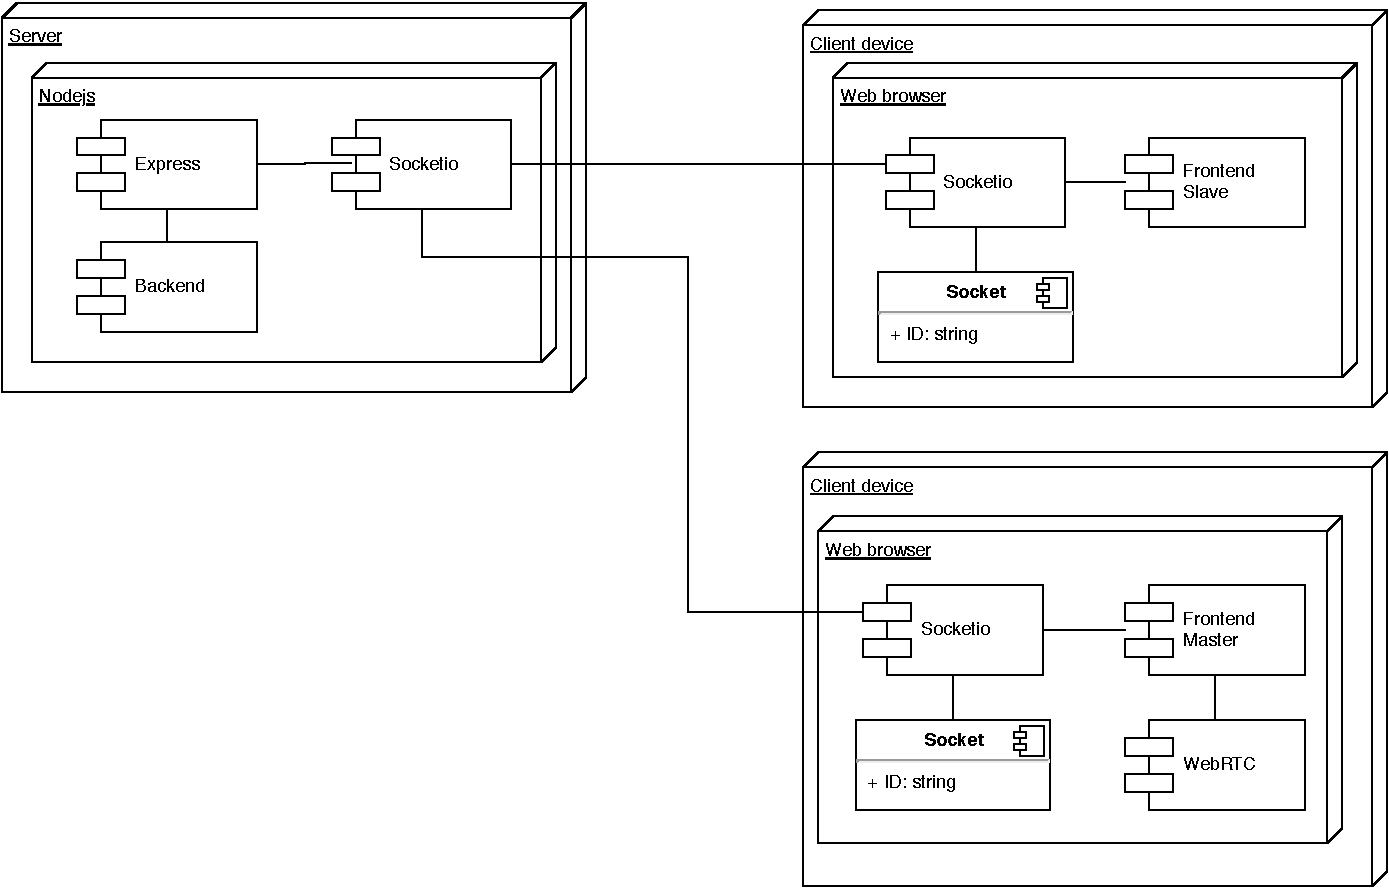
\includegraphics[width=\textwidth]{figures/deployment}
	\caption{Deployment diagram of the multiscreen casting framework.} 
	\label{fig:deployment}
\end{figure}

\exampletext{We rely on webrtc~\cite{website:webrtc} to collect a client-side video stream. This module offers the necessary tools for serialization, i.e., as a base64 encoded string. Serialization is required for transmission~\cite{website:serialization}. Server-side the backend code will process the image. In our demo we broadcast the image by sending it to all slaves. Slaves and masters can be reached by the server, as we use the concept of a namespace~\cite{website:namespaces}. A namespace can be used to group clients with a similar role, and broadcast to them. 

A socket is assigned a unique identifier by Socketio. This identifier can be used to emit messages from the server to a specific client. A list of connected clients is available through the API of Socketio \cite{website:socketio-clients}.}

\section{Algorithms}\label{sec:technical-analysis}

\note{($\approx$ 1 page. Depending on necessity)}
\exampletext{\textit{When you design or use an algorithm you should be able to explain how well it performs and if it satisfies the requirements. Often there will be alternatives or system parameters that need to be chosen. We want to know why you chose a specific set of parameters, or why you chose an approach over another. We supply some example text of last year.}}



\subsection{Scherm identificatie met barcodes}

\subsubsection{Algemene uitleg}

De identificatie van schermen gebeurt aan de hand van een kleuren barcode. Het slave-scherm zal binnen zijn rand(gebruikt voor edge detection) een herhalend patroon van 5 kleuren en wit tonen. Aan de hand van de volgorde kan een unieke code per scherm gelezen worden en zo is elk scherm duidelijk gedefinieerd. De 5 kleuren zijn speciaal gekozen om zo ver mogelijk uit elkaar te liggen in het HSL spectrum om fouten lezingen te vermijden. Ze dragen elk een cijfer van 1 tot en met 5 en worden maar één keer gebruikt in de barcode. Dit zorgt ervoor dat we in theorie een totaal van $5!$ ($=120$) verschillende schermen op één moment kunnen detecteren. Het herhalend patroon geeft ons de mogelijkheid om fouten te vermijden. Na het vinden van het scherm zelf (zie sectie 3.2) zal de barcode gelezen worden. Indien een reflectie of een overlap plaatsvind kan een stuk van het scherm bedekt zijn. De scanner() zal het midden van het scherm lezen in rechte lijn (volgens de orientatie), aangezien een stuk bedekt is zal deze blijven gaan tot hij 5 kleuren en wit tegenkomt. Zo niet, zal de lijst met codes leeggemaakt worden en verder gaan. Het herhalend patroon is dus essentieel aan het correct inlezen.

\begin{figure}
\centering

\includegraphics[scale=0.1]{barcode}
\caption{Voorbeeld van een barcode met 6 herhalingen.} 
\label{fig:barcode}
\end{figure}



\subsubsection{Data set}

Om het scanner() algorithme te testen hebben we een aantal foto's genomen vanop verschillende afstanden, met verschillende computers (kleuren kunnen afwijken van scherm tot scherm) en met verschillende aantal barcodes dat op het scherm past. Aangezien een herhalend patroon gebruikt wordt kan men kiezen hoeveel er per scherm staan, dit kan van 3 tot 15 gaan (meer heeft niet veel zin want het onderschijden van kleuren wordt lastig).

\subsubsection{Experiments}\label{sec:experimenten}

\subsection{Image}
\subsubsection{Algemene uitleg}
\subsubsection{Data set}
\subsubsection{Experiments}

\section{Testen}
\subsection{Algemeen concept}
De testen maken gebruik van een simpele server waar clients op kunnen verbinden. De client kan vervolgens het absolute tijdverschil meten met een atomische wereldklok.

Eerst en vooral is er een vertraging tussen een aangesloten client en de server, de {\it ping}. Dit is gemeten in milliseconden. De testen meten de vertraging door een bericht met de actuele tijd te verzenden van de server naar de client, en terug. De vertraging is dan de verzonden tijd afgetrokken van de actuele tijd waarmee de ping verkregen is.
In figuur \ref{ping} is de informatieoverdracht zichtbaar. De server berekent de servertijd (TS1) door middel van een API die de exacte wereldtijd teruggeeft, verzonden naar de client en teruggekregen. De uiteindelijke ping is: \[ping = TS2 - TS1\] met TS2 de actuele tijd berekent in de server TS2

\begin{figure}[h]
\centering
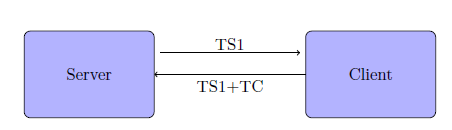
\includegraphics[scale=0.8]{img/img.png}
\caption{Ping} \label{ping}
\end{figure}


Het is niet gegarandeerd dat de klokken van de clients allemaal gesynchroniseerd zijn met de server. Bij het terug verzenden van de client naar de server wordt de clienttijd (TC) bij het bericht gezet.  Met deze TC en de berekende {\it ping} is het mogelijk het tijdsverschil tussen de client en de server te bepalen ($DeltaTime$).
\[DeltaTime = (TC+ping/2) - TS2\]
Deze data wordt vervolgens tussen verschillende browsers en besturingssystemen vergeleken.

\subsection{UDP vs TCP}

UDP heeft in tegenstelling tot TCP geen gevestigde verbinding nodig tussen bijvoorbeeld server en client. TCP zal garanderen dat data correct aankomt door middel van foutopsporing en zal ook in de goede volgorde binnenstromen. Om geen pakketten te verliezen zal TCP deze in een {\it receive buffer} steken en zal de applicatie de ontvangen data pas lezen als ze er klaar voor is. Tegenover UDP waar de data continu zal binnenstromen, ontvangen of niet. Deze zal ook niet aan foutopsporing doen en de juiste volgorde niet gegaranderen. Het is duidelijk dat UDP veel sneller is doordat deze minder stappen en controle bevat. Dit is ook de reden dat het NTP protocol UDP zal gebruiken in plaats van TCP. Het is logisch dat voor een simpele synchronisatie tussen client en server geen complex protocol nodig is. Socket.io gebruikt het TCP protocol in de browser voor veiligheidsredenen.

\subsection{Drift en skew}

Drift zal ervoor zorgen dat een klok niet meer synchroon met zijn oorspronkelijke referentie loopt. Windows lost dit op met een wekelijkse resync (het tijdsverschil zal dus op een sawtooth diagram lijken) terwijl Mac OSX rekening zal houden met de klok skew en andere hardware invloeden om zo beter synchroon te blijven.
Klok skew is het verschil van tijd van een kloksignaal tussen 2 componenten binnen een systeem(zie figuur \ref{skew1} \cite{skew}).

Het tijdsverschil van een windows computer en een atoomklok is gedurende 25 minuten gemeten (zie figuur \ref{drift}). De trendlijn is door de grafiek getrokken en het is duidelijk dat er geen effect ervan te zien is. Over langere tijdsperiode zal de drift groter worden, maar voor de animatie zal dit verwaarloosbaar zijn aangezien het onwaarschijnlijk is dat iemand dagenlang deze zal laten afspelen.

\begin{figure}[H]
\centering
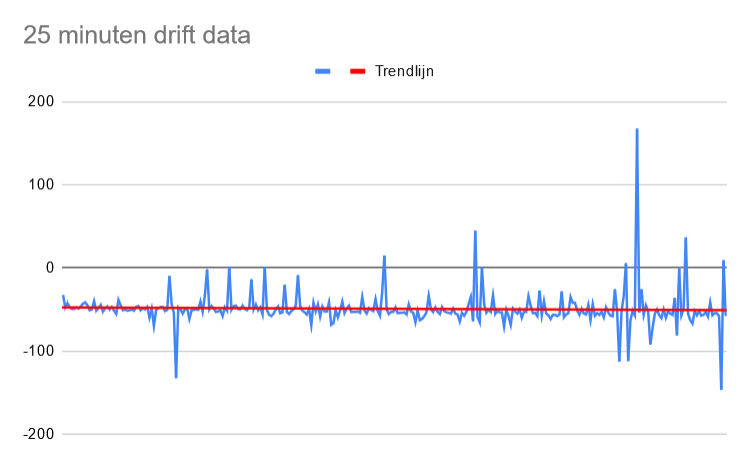
\includegraphics[scale=0.3]{img/drift.png}
\caption{Drift} \label{drift}
\end{figure}

\begin{figure}[H]
\centering
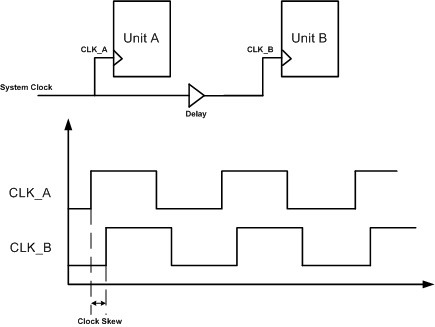
\includegraphics[scale=0.7]{img/skew.jpg}
\caption{Skew} \label{skew1}
\end{figure}


Klok skew kan problemen geven voor correct timings, en zoals eerder vermeld zal OSX dit tegen gaan via software. We zullen niet dieper gaan over de problemen van skew en OSX. 


\subsection{Analyse van de data}
\label{analyse}
Het is duidelijk dat er op elk soort systeem een afwijking gemeten wordt tegenover de referentieklok. Bij sommige operating systems al een groter verschil dan de andere, maar de reden waarom is niet altijd te verklaren of vrijgegeven en zullen hier dus niet verder op in gaan. Elk systeem wordt door het operating system zelf voldoende gesynchroniseerd met een server-klok als referentie en zou in principe maar een paar miliseconden mogen afwijken van deze referentieklok. De fout wordt pas waargenomen in de metingen van het verschil tussen de twee klokken over een netwerk. In deze situatie wordt er een poging gedaan om het verschil tussen device-klok en server-klok te vergelijken door de ping mee in rekening te brengen. De drift van beide klokken gaan over deze tijdsspanne minimaal zijn en gaan geen invloed hebben op deze verschillen. Bij de testen werd ook de gemiddelde ping en standaarduitwijking van de ping per test opgeslagen. Uit deze waarden valt af te leiden dat er bij grote pingfluctuaties ook een grote standaarduitwijking mee gepaard ging en wijst naar inconsistenties binnen het netwerk van ofwel de client ofwel de belasting op de server en is er bijgevolg meer kans op een grotere fout binnen de vergelijking van de klokken. 

\begin{figure}[H]
	\centering
	\begin{subfigure}{.5\textwidth}
		\centering
		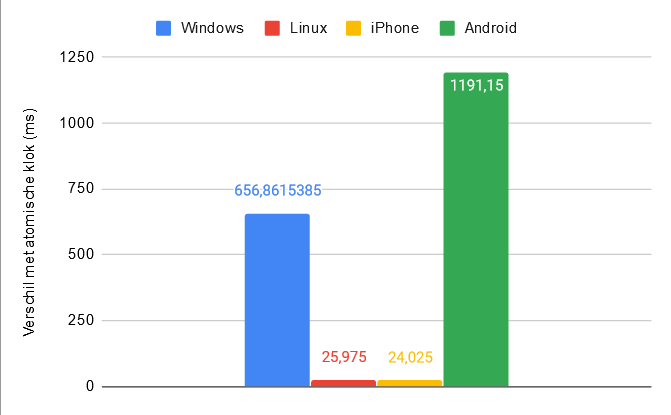
\includegraphics[width=.95\linewidth]{img/mediaan.png}
		\caption{Mediaan van tijdsverschil van elk device.}
		\label{fig:mediaan}
	\end{subfigure}%
	\begin{subfigure}{.5\textwidth}
		\centering
		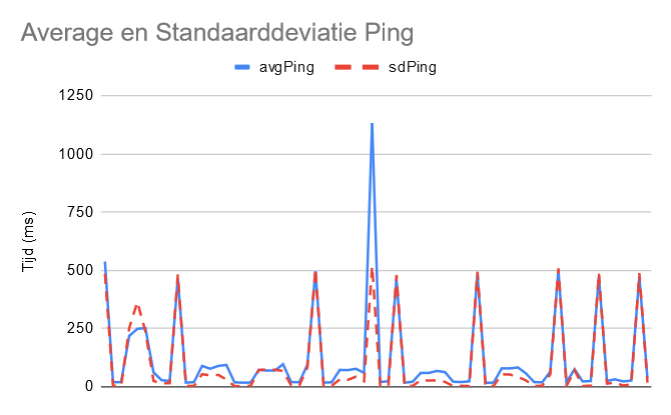
\includegraphics[width=.95\linewidth]{img/ping_results.png}
		\caption{Gemiddelde en standaarduitwijking van de ping met de server. }
		\label{fig:avgPing}
	\end{subfigure}
	\caption{Resultaten van de testen}
	\label{fig:results}
\end{figure}

In figuur \ref{fig:avgPing} is het duidelijk zichtbaar dat er een pieken zijn met hoge standaardafwijkingen. Dit wilt zeggen dat er heel grote fluctuaties zijn in de ping tijdens het synchronisatie proces met 10 opmetingen. Hiermee is de gesynchroniseerde tijd een afwijking hebben met de werkelijke tijd tot ($maxPing - minPing$).





















\section{Besluit}\label{sec:besluit}
 
Uit de bevindingen is gebleken dat de interpretatie van kleur sterk afhankelijk is van de manier waarop kleur wordt voorgesteld en de omgevingsfactoren die hierbij aanwezig zijn. Enerzijds speelt de kleurruimte waarin een kleur wordt voorgesteld een grote rol bij de detectie. Van de verschillende kleurruimten die bekeken zijn, is er niet een die eenduidig beter is dan de andere. Beiden hebben hun voordelen, zo is HSL beter voor de detectie van alle kleuren dan RGB. Maar de detectieratio van zwart en wit is dan wel weer aannoemelijk beter in RGB dan in HSL.  Anderzijds spelen omgevingsfactoren ook een belangrijke rol bij de detectie van de kleuren. Hiervoor werd gekeken naar zowel de omgeving, de lichtinval en de helderheid van het scherm. De belangrijkste bevindingen hierbij hebben te maken met de lichtinval en de omgeving. Door lichtinval komt er bij artificieel licht extra rood in de kleuren door de rode schijn die het licht achterlaat. Hoe groter de omgeving, hoe meer de kleuren fout gedetecteerd gaan worden. Dit is te wijten aan het feit dat de camera hierbij op de omgeving gaat focussen in plaats van op het scherm. Tot slot is ook gebleken dat helderheid geen groot effect heeft op de detectie.

%%%%%%%%%%%%%%%%%%%%%%%%%%%%%%%%%%%%%%
%%%%%%%%%%%%%%%%%%%%%%%%%%%%%%%%%%%%%%

%%%%%%%%%%%%%%%%%%%%%%%%%%%%%%%%%%%%%%

%%%%%%%%%%%%%%%%%%%%%%%%%%%%%%%%%%%%%%
\bibliographystyle{plain}
\bibliography{bibliography}

% \bigskip

% \vspace*{\fill}

% %% This is a basic score card
% %% please fill in your team number and name
% %% don't touch the rest!
% %%%%%%%%%%%%%%%%%%%%%%%%%%%%%%%%%%%%%%
% \noindent
% %\mbox{}\hfill
% \begin{tabular}{*3l}
% \toprule
% \multicolumn{3}{l}{\large\textbf{Evaluation card: Team <number> <name>}} \\
% Criterion & Score (/10) & Remarks \hspace{6cm} \\
% \midrule
% References \\
% Algorithm descriptions \\
% Correctness \\
% Clearness \\
% Writing style \\
% Conciseness \\
% Self-evaluation \\
% Informative figures \\
% Tests \\
% \bottomrule
% \hline
% \end{tabular}

\end{document}